\documentclass[../Dissertation.tex]{subfiles}
\begin{document}
\subsection{Results}


\iffalse
\begin{tabular}{l|l|c|c|c}
\multicolumn{2}{c}{\underline{Back Test Violations}}&\multicolumn{2}{c}{Time Horizon}&\\
\cline{3-4}
\multicolumn{2}{c|}{}&1&10&\multicolumn{1}{c}{Total}\\
\cline{2-4}
\multirow{2}{*}{Confidence}& 0.95 & $24260$ & $11280$ & $35540$\\
\cline{2-4}
& 0.99 & $7160$ & $900$ & $8060$\\
\cline{2-4}
\multicolumn{1}{c}{} & \multicolumn{1}{c}{Total} & \multicolumn{1}{c}{$31420$} & \multicolumn{    1}{c}{$12180$} & \multicolumn{1}{c}{$43600$}\\
\end{tabular}


\begin{tabular}{l|l|c|c|c}
\multicolumn{2}{c}{\underline{Stress Test Violations}}&\multicolumn{2}{c}{Time Horizon}&\\
\cline{3-4}
\multicolumn{2}{c|}{}&1&10&\multicolumn{1}{c}{Total}\\
\cline{2-4}
\multirow{2}{*}{Confidence}& 0.95 & $21420$ & $30020$ & $51440$\\
\cline{2-4}
& 0.99 & $6960$ & $6220$ & $13180$\\
\cline{2-4}
\multicolumn{1}{c}{} & \multicolumn{1}{c}{Total} & \multicolumn{1}{c}{$28380$} & \multicolumn{    1}{c}{$36240$} & \multicolumn{1}{c}{$64620$}\\
\end{tabular}
\fi

\paragraph{Diversification}
First, let us consider what impact increasing the number of assets in our portfolio had on our VaR estimates.
In figure~\ref{fig:diversification} on page~\pageref{fig:diversification}, we can see the average VaR as a percentage against the number of assets.
Increasing the number of assets in our portfolio decreases our exposure to risk.
Thus we demonstrate the benefits of diversification.
						\begin{wrapfigure}{r}{0.5\textwidth}
								\caption{Diversification}
								\label{fig:diversification}
								\centering
								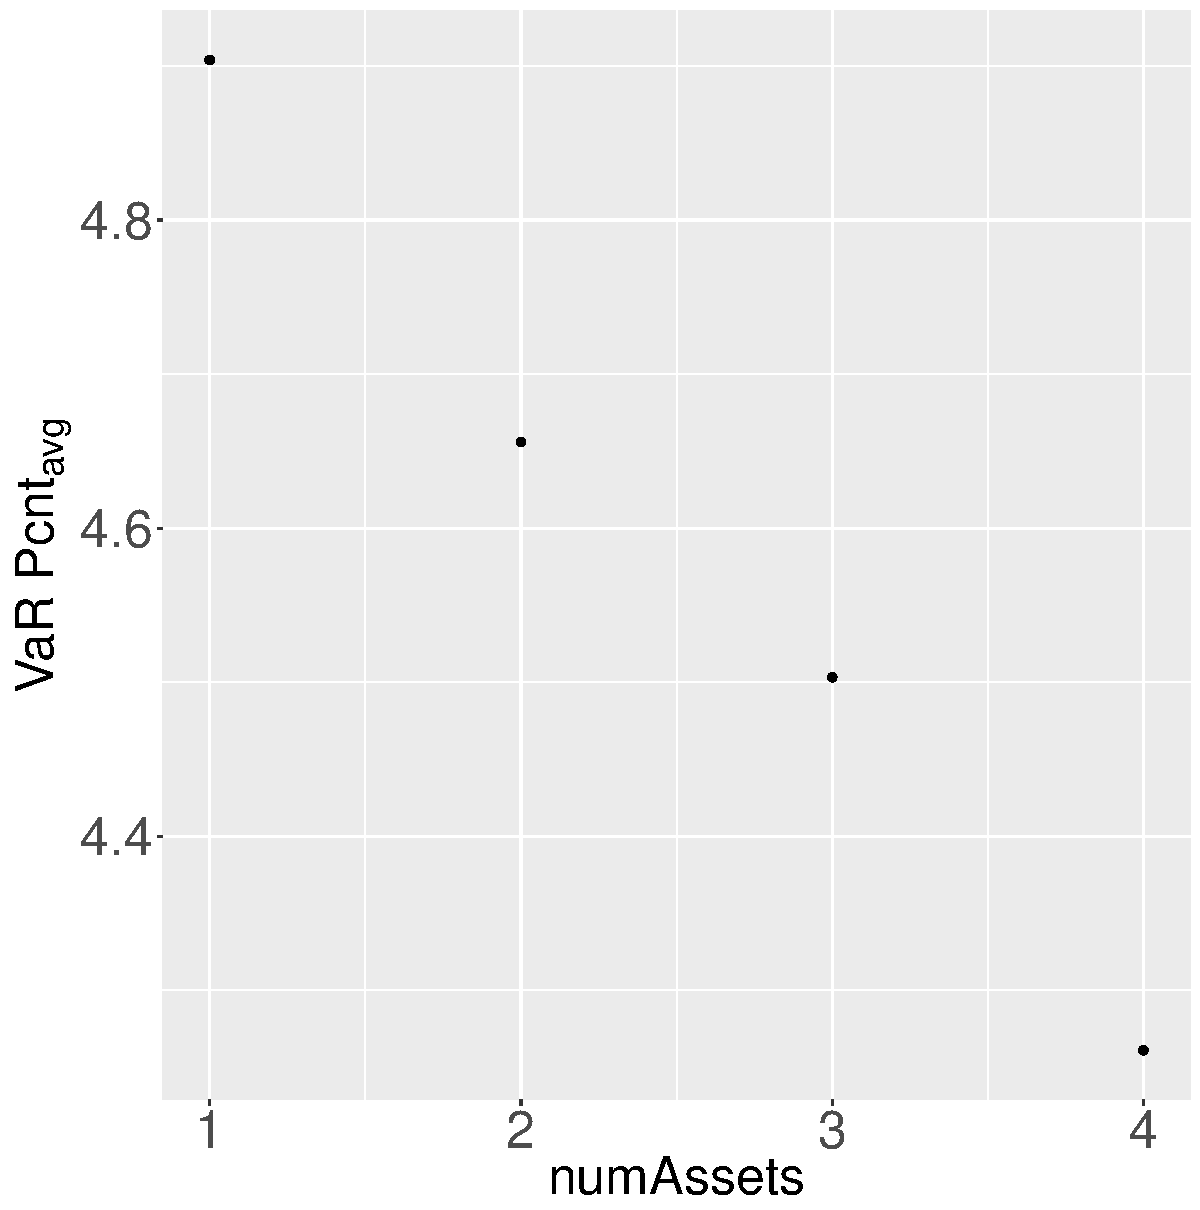
\includegraphics[width=0.48\textwidth]{./assets/Diversification.pdf}
						\end{wrapfigure}
\paragraph{Non-Rejection Intervals}	
In our back test, we defined non-rejection intervals using coverage tests.
The size of these intervals were varied depending on the chosen significance level.		
In figure~\ref{fig:ConfidenceInterval} on page~\pageref{fig:ConfidenceInterval}, we can see two sets of intervals: the set with the mean at 50 represents our intervals at  95\% confidence.
The other set has a mean at 10 and represents our intervals at 99\% confidence.
The range between the intervals is larger at 95\%.
We would expect that the number of violations that land within the non-rejection interval to be much smaller at 99\% than at 95\%.

In figure~\ref{fig:ViolationsBoxplots} on page~\ref{fig:ViolationsBoxplots} we see the distribution of the violations with respect to confidence during Back Testing and Stress Testing.
It is apparent that our during our Stress Test, we an increase in violations.
This suggests that our VaR measures are not particularly affective during crises.
But nonetheless, even during Back Testing, the mean violations fall below our expected number of violations.
It is even below the lower bound of our widest non-rejection interval at 95\%.
If we must widen this interval, then this might suggest that our VaR estimates are not particularly accurate.

\begin{figure}[H]
\centering
\begin{minipage}{0.5\textwidth}
  \centering
  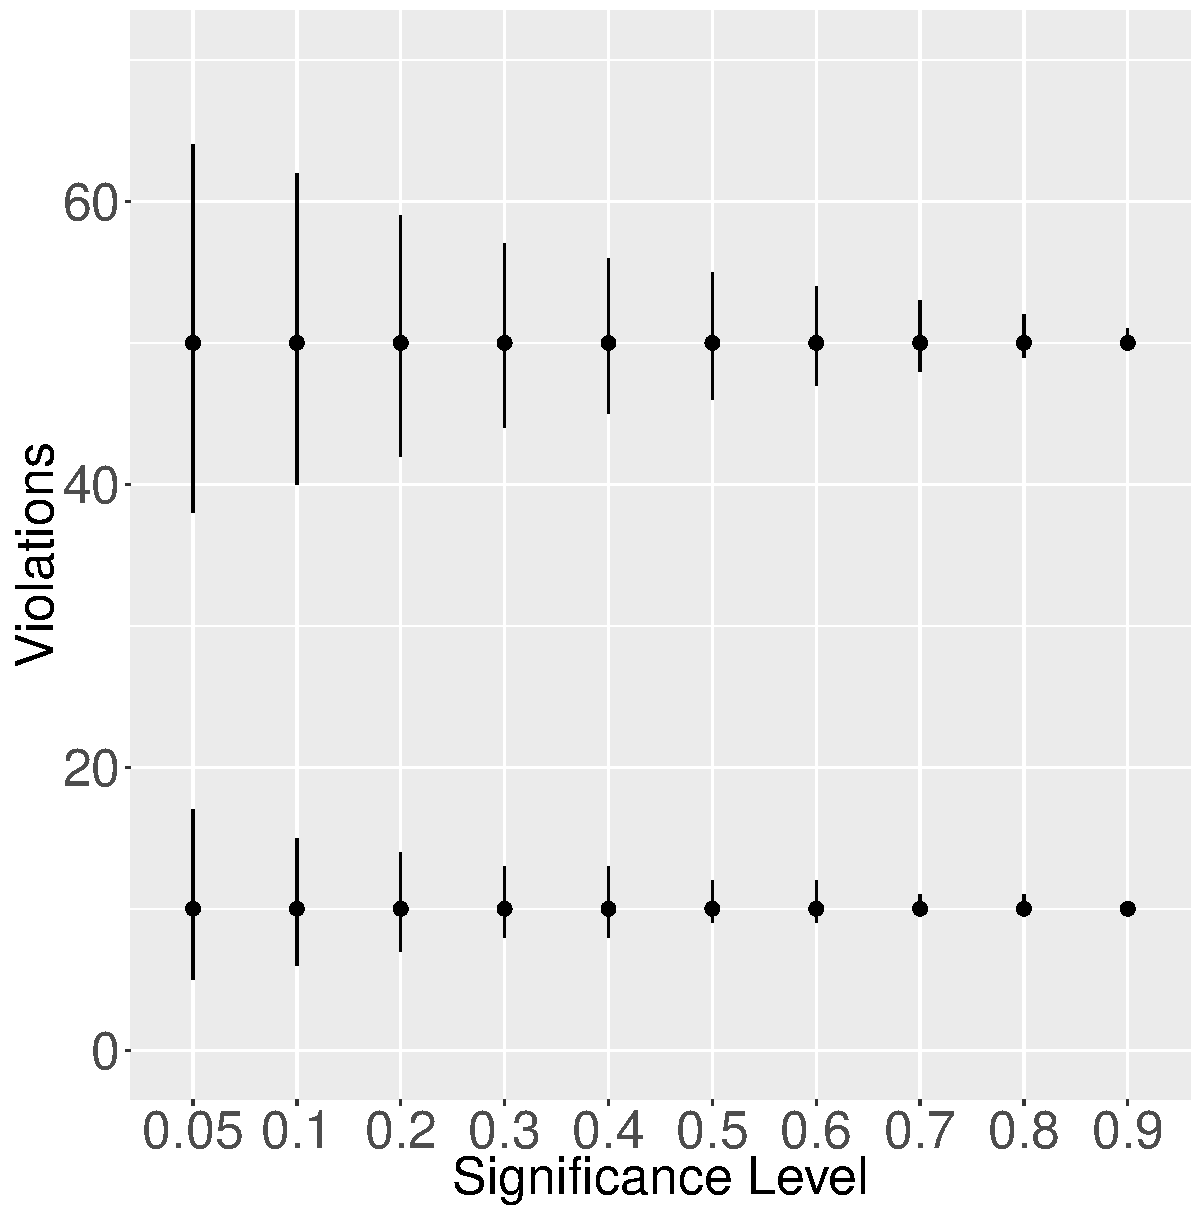
\includegraphics[width=\linewidth]{./assets/CoverageIntervals.pdf}
  \captionof{figure}{Non-Rejection Intervals \\at 95\% and 99\%}
  \label{fig:ConfidenceInterval}
\end{minipage}%
\begin{minipage}{.5\textwidth}
  \centering
  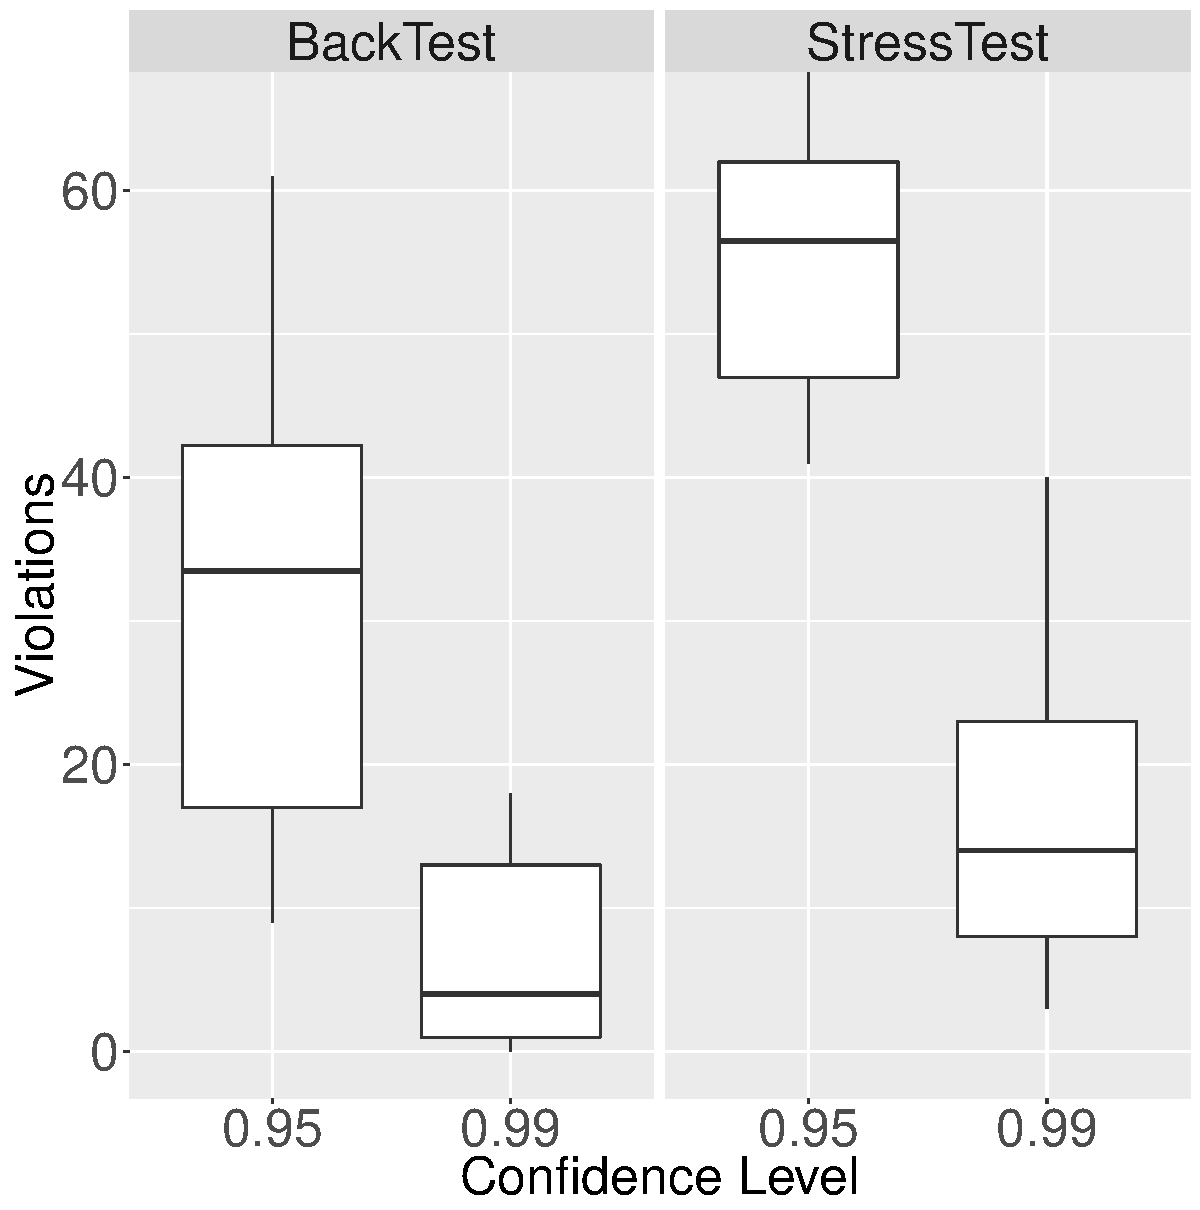
\includegraphics[width=\linewidth]{./assets/ViolationsBoxplots.pdf}
  \captionof{figure}{Distribution of Violations \\at 95\% and 99\%}
  \label{fig:ViolationsBoxplots}
\end{minipage}
\end{figure}					

In figure~\ref{fig:ViolationsKeepsT1} on page~\pageref{fig:ViolationsKeepsT1}, we see the distribution of our violations in a dot plot at a time horizon of 1 day. 
In red are the the violations that fall within the non-rejection interval.
The blue violations fall outside this interval.
Interestingly, the maximum number of violations that occurred during the Stress Test is not all that much higher than during the Back Test.
Comparing this distribution against the box plot in figure~\ref{fig:ViolationsBoxplots}, we see that the increase in violations is largely due to the exclusion of data from the experiments that used a 10 day time horizon.
We can even see that at the 95\%  confidence level we have no rejected violations during the Stress Test at a significance level of 5\%, which gives us an indication of how confident and accurate we are being.

In Back Testing, there are noticeable gaps in the distribution where we should have some non-rejected violations.
It is possible that there is a gap in the data.
More worryingly, it could suggest that the past five years of market conditions are much worse than the period in which the Stress Test takes place.
						\begin{wrapfigure}{r}{0.5\textwidth}
						%\begin{figure}
								\caption{Accepted/Rejected Violations}
								\label{fig:ViolationsKeepsT1}
								\centering
								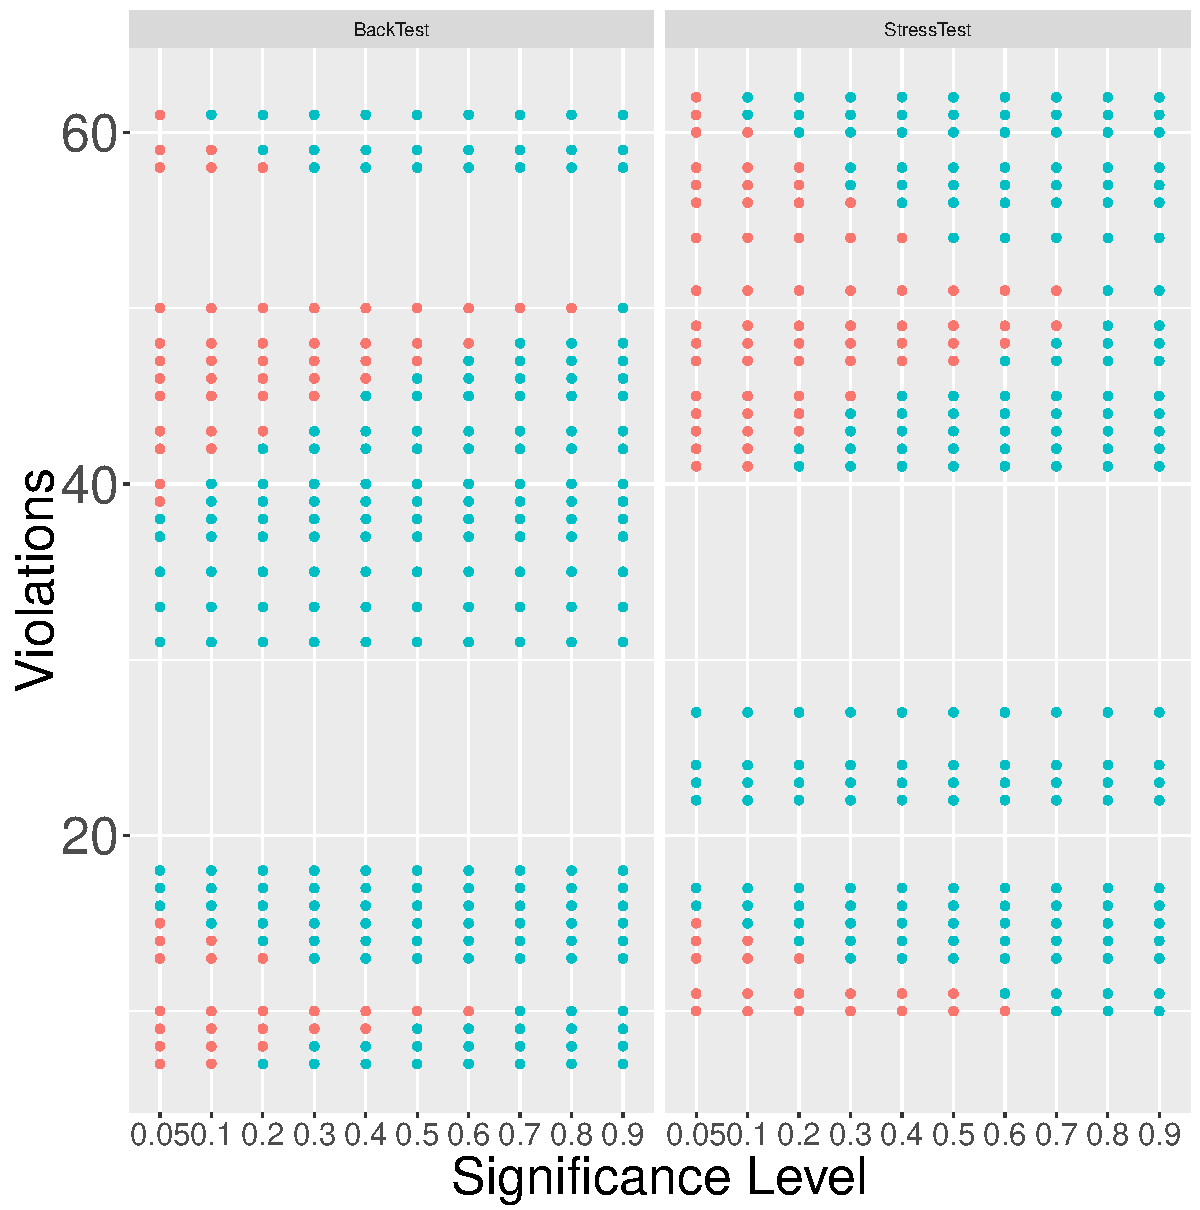
\includegraphics[width=0.5\textwidth]{./assets/ViolationsKeepsT1.pdf}
								%\end{figure}
						\end{wrapfigure}



\paragraph{Which Measure?}

Now, having tested seven different VaR measures, we must ascertain whether their performance differs and even whether one measure is definitively better than the others.
We would expect the Analytical approach to perform similarly to the Monte Carlo approach as they both make the same underlying probabilistic assumptions.
The only difference being is how they go about producing their estimates.

In figure~\ref{fig:nonrejectionviolations} on page~\pageref{fig:nonrejectionviolations}, we can see the number of non-rejected violations for each measure.
We see more non-rejections during the Stress Test, which is consistent with our other observations.
In either case, the two equal-weighted measures have performed the worst.
Confusingly, Analytical GARCH is in the bottom three during Back Test but is in the top three during Stress Test.
Both EWMA measures had among the highest levels of non-rejections; in particular for the Monte Carlo EWMA measure.

\begin{figure}
\caption{Measures/Non-Rejected Violations}
\label{fig:nonrejectionviolations}
\centering
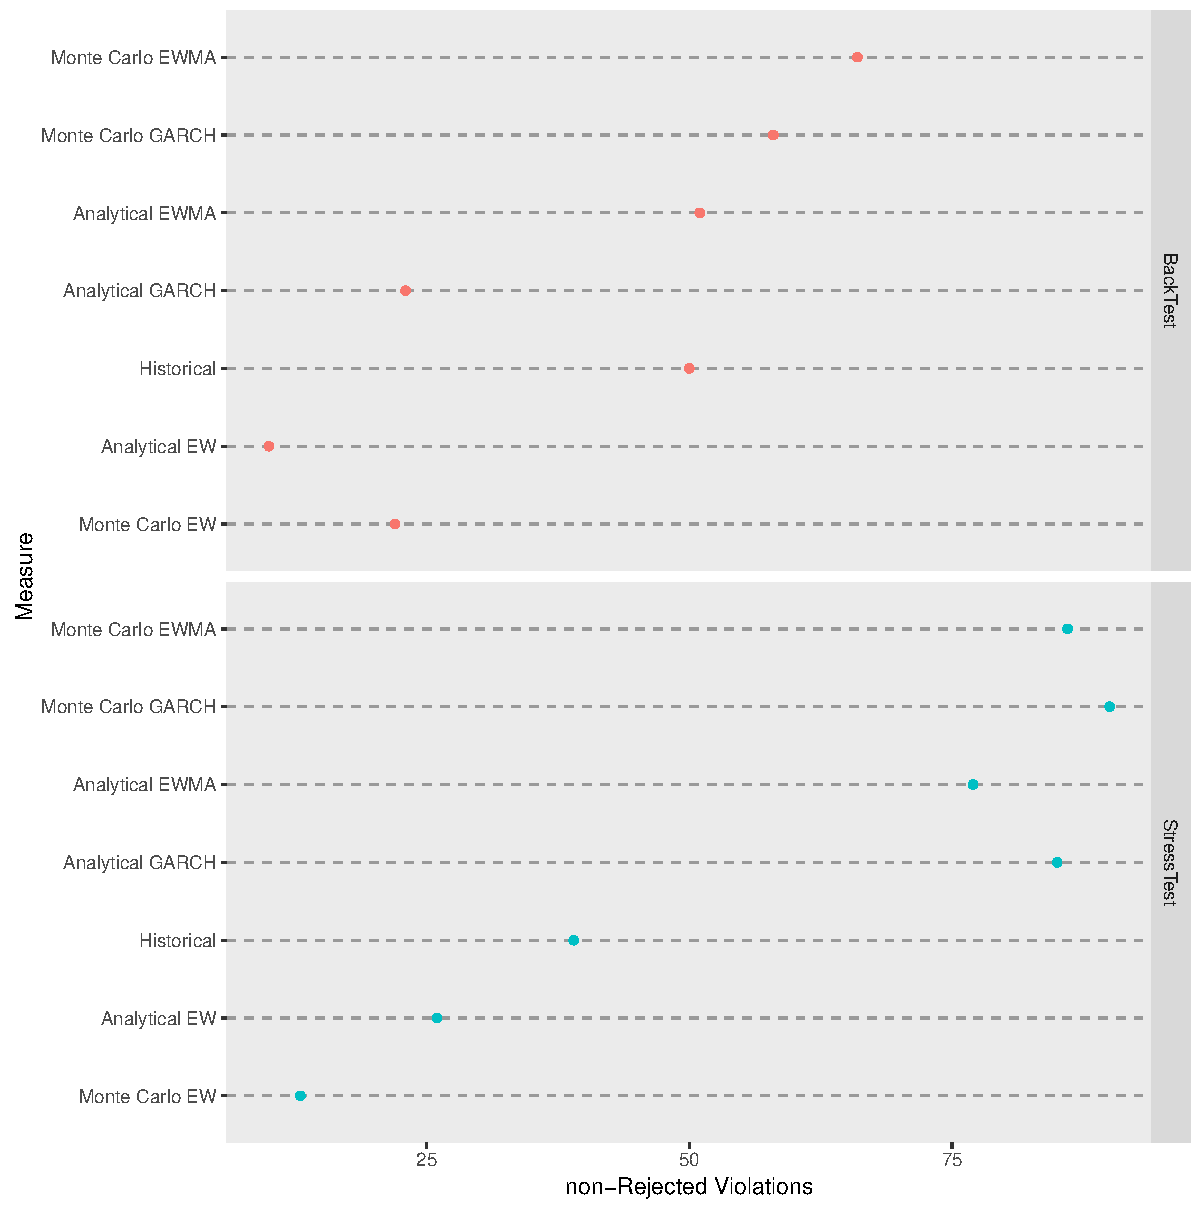
\includegraphics[width=\textwidth]{./assets/nonrejectionviolations.pdf}
\end{figure}
\end{document}